\centering
\section*{\underline{Allgemein}}

\begin{tikzpicture}[remember picture, overlay]

% ---- ERSTE REIHE: Am Seitenursprung starten
\setlength{\rowheight}{30mm}

    % A1) Erste Kachel oben links
    \setlength{\cellwidth}{48mm}
    \Tile{A1}{([xshift=10mm,yshift=-18mm]current page.north west)}{\cellwidth}{\rowheight}
        {
            \vspace{-\TileSep}
            \titlerm{Kräfte, Nickmoment}\\ \vspace{-2mm}
            \begin{align*}
                A &= \frac{\rho_\infty}{2}\,U_\infty^2\,S\,c_A \\
                W &= \frac{\rho_\infty}{2}\,U_\infty^2\,S\,c_W \\
                M &= \frac{\rho_\infty}{2}\,U_\infty^2\,S\,c_M\,t
            \end{align*}
        }{0}{1}{1}{0}

    % B1) Zweite Kachel rechts anbauen
    \setlength{\cellwidth}{40mm}
    \Tile{B1}{(A1.north east)}{\cellwidth}{\rowheight}
        {
            \vspace{-\TileSep}
            \titlerm{Beiwerte}\\ \vspace{-2mm}
            \begin{align*}
                c_a &= \left(\frac{\text{d}c_a}{\text{d}\alpha}\right)_\text{2D}\,\alpha_e \\[1.0ex]
                c_p &= \frac{p - p_\infty}{\frac{\rho_\infty}{2}\,U_\infty^2}
            \end{align*}
        }{0}{1}{1}{0}

    % C1) Dritte Kachel rechts anbauen
    \setlength{\cellwidth}{55mm}
    \Tile{C1}{(B1.north east)}{\cellwidth}{\rowheight}
        {
            \vspace{-\TileSep}
            \titlerm{Flügelmaße}\\ \vspace{-2mm}
            \begin{align*}
                \Lambda = \frac{b^2}{S} = \frac{2\,b}{l_\text{i}+l_\text{a}}\qquad \lambda = \frac{l_\text{a}}{l_\text{i}} \\[1.0ex]
                \text{Trapezflügel:}\ \ S = b\,\frac{l_\text{i}+l_\text{a}}{2}~
            \end{align*}
        }{0}{1}{1}{0}
    
    % D1) Vierte Kachel rechts anbauen
    \setlength{\cellwidth}{47mm}
    \Tile{D1}{(C1.north east)}{\cellwidth}{\rowheight}
        {
            \vspace{-\TileSep}
            \titlerm{Mach-Zahl}\\ \vspace{-2mm}
            \begin{equation*}
                \text{Ma}_\infty = \frac{U_\infty}{\sqrt{\kappa\,R\,T_\infty}}
            \end{equation*}
            \begin{equation*}
                \kappa = \text{1,4}\qquad R = \text{287,1}\,\tfrac{\text{J}}{\text{kg}\cdot\text{K}}
            \end{equation*}
        }{0}{0}{1}{0}

% ---- ZWEITE REIHE: Am Seitenursprung starten
\setlength{\rowheight}{52mm}

    % A2) Erste Kachel unten anbauen
    \setlength{\cellwidth}{88mm}
    \Tile{A2}{(A1.south west)}{\cellwidth}{\rowheight}
        {
            \titlerm{Krit. Mach-Zahl / Druckbeiwert}\\[1.0ex]
            $\text{Ma}^*_\infty$ ist die Anströmmachzahl, bei der lokal erstmals $\text{Ma}^*_\text{lokal} \geq 1$ auftritt. Mit Bernoulli:\\
            $\text{Ma}_\text{\,lokal,\,max}$ an der Stelle von $c^*_{p\,\text{lokal,\,min}}$
            \begin{align*}
                c_{p,\text{min}} = c^*_p = \frac{2}{\kappa\,\text{Ma}^2_\infty}\,\left[\left(\frac{2}{\kappa+1}+\frac{\kappa-1}{\kappa+1}\,\text{Ma}^2_\infty\right)^\frac{\kappa}{\kappa-1}-1\right]
            \end{align*}
            Näherung für dünne Profile (schwach angestellt):
            \begin{equation*}
                c_{p,\text{min}} = c^*_p \approx \frac{2}{\kappa+1}\,\frac{\text{Ma}^2_\infty-1}{\text{Ma}_\infty^*}
            \end{equation*}
        }{0}{1}{1}{0}

    % B2) Zweite Kachel rechts anbauen
    \setlength{\cellwidth}{102mm}
    \Tile{B2}{(A2.north east)}{\cellwidth}{\rowheight}
        {
            \titlebf{Winkel am Flügelprofil}\\ \vspace{-1mm}
            \begin{minipage}{0.55\cellwidth-\TileSep}
                \centering
                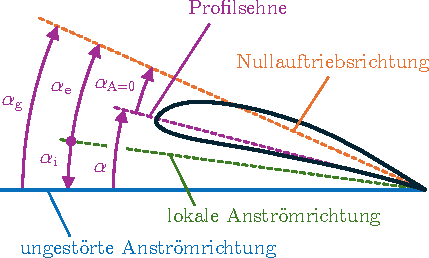
\includegraphics[width=0.9\textwidth]{images/profilwinkel.pdf}
            \end{minipage}%
            \begin{minipage}{0.45\cellwidth-\TileSep}
                \centering
                \begin{align*}
                    \alpha &= \alpha_\text{e} + \alpha_\text{i} + \alpha_\text{A=0} \\
                    \alpha_\text{e} &= \alpha_\text{g} - \alpha_\text{i}
                \end{align*}
                \begin{align*}
                    \alpha            &= \text{Anstellwinkel}       \\
                    \alpha_\text{A=0} &= \text{Nullauftriebswinkel} \\
                    \alpha_\text{e}   &= \text{Effektiver AW}       \\
                    \alpha_\text{g}   &= \text{Geometrischer AW}    \\
                    \alpha_\text{i}   &= \text{Induzierter AW}
                \end{align*}
            \end{minipage}
        }{0}{0}{1}{0}

\end{tikzpicture}

\vspace{78mm}
\centering
\section*{\underline{Skeletttheorie}}

\begin{tikzpicture}[remember picture, overlay]

% ---- ERSTE REIHE: Am Seitenursprung starten
\setlength{\rowheight}{30mm}

    % A1) Erste Kachel unten anbauen
    \setlength{\cellwidth}{98mm}
    \Tile{A1}{([xshift=10mm,yshift=-112mm]current page.north west)}{\cellwidth}{\rowheight}
        {
            \vspace{-\TileSep}
            \titlerm{Koeffizienten}\\ \vspace{-3mm}
            \begin{minipage}{0.42\cellwidth-\TileSep}
                \centering
                \begin{align*}
                    A_0 &= \alpha^* + \alpha_0 \\
                    A_1 &= 2\,\left(\alpha_2 - \alpha\right) = 4\,\frac{f}{t} \\
                    A_2 &= -3\,\alpha_2
                \end{align*}
            \end{minipage}%
            \begin{minipage}{0.58\cellwidth-\TileSep}
                \centering
                \begin{align*}
                    A_0 &= \alpha^* + \alpha_0 = \alpha^* - \frac{1}{\pi}\,\int\limits_0^\pi \frac{\text{d}z}{\text{d}x}\,\text{d}\Phi \\
                    A_n &= -\frac{2}{\pi}\,\int\limits_0^\pi\frac{\text{d}z}{\text{d}x}\,\cos\left(n\,\Phi\right)\,\text{d}\Phi
                \end{align*}
            \end{minipage}
        }{0}{1}{1}{0}

    % B1) Zweite Kachel rechts anbauen
    \setlength{\cellwidth}{40mm}
    \Tile{B1}{(A1.north east)}{\cellwidth}{\rowheight}
        {
            \vspace{-\TileSep}
            \titlerm{Kräfte}\\ \vspace{-3mm}
            \begin{align*}
                A &= G = \frac{\pi}{4}\,b\,\rho\,U_\infty\,A_1 \\[1.5ex]
                W_\text{i} &= \frac{\pi}{8}\,\rho\,\sum\limits_{n=1}^M\left(n\,A_n^2\right)
            \end{align*}
        }{0}{1}{1}{0}

    % C1) Dritte Kachel rechts anbauen
    \setlength{\cellwidth}{52mm}
    \Tile{C1}{(B1.north east)}{\cellwidth}{\rowheight}
        {
            \vspace{-\TileSep}
            \titlerm{Position der max. Wölbung}\\ \vspace{-2mm}
            \begin{equation*}
                \frac{\text{d}\bar{z}}{\text{d}\bar{x}} = 0~(\text{maximum von }\bar{z}(\bar{x}))
            \end{equation*}
            \begin{equation*}
                \frac{f}{t} = \frac{A_1}{4}
            \end{equation*}
        }{0}{0}{1}{0}

% ---- ZWEITE REIHE: Am Seitenursprung starten
\setlength{\rowheight}{38mm}

    % A2) Erste Kachel unten anbauen
    \setlength{\cellwidth}{95mm}
    \Tile{A2}{(A1.south west)}{\cellwidth}{\rowheight}
        {
            \titlerm{Beiwerte}\\ \vspace{3mm}
            \begin{minipage}{0.47\cellwidth-\TileSep}
                \centering
                \vspace{-3mm}
                \begin{align*}
                    c_a &= \pi\,\left(2\,A_0 + A_1\right)\\
                    \Delta c_p &= c_{p,\text{u}} - c_{p,\text{o}} = 2\,\frac{\gamma(\bar{x})}{U_\infty}
                \end{align*}
            \end{minipage}%
            \vline
            \begin{minipage}{0.53\cellwidth-\TileSep}
                \centering
                \vspace{-3mm}
                \begin{align*}
                    c_{m,\text{VK}} &= -\frac{\pi}{4}\,\left(2\,A_0 + 2\,A_1 + A_2\right) \\
                    c_{m,\sfrac{t}{4}} &= c_{m,\text{VK}} + \frac{c_a}{4}
                \end{align*}
            \end{minipage}
            \begin{equation*}
                \frac{\text{d}c_a}{\text{d}\alpha} = 2\,\pi~;\quad \frac{\text{d}c_m}{\text{d}\alpha} = 0
            \end{equation*}
        }{0}{1}{1}{0}

    % B2) Zweite Kachel rechts anbauen
    \setlength{\cellwidth}{95mm}
    \Tile{B2}{(A2.north east)}{\cellwidth}{\rowheight}
        {
            \titlebf{Nullauftrieb und -moment}\\ \vspace{2mm}
            \begin{minipage}{0.46\cellwidth-\TileSep}
                \centering
                \begin{align*}
                    \alpha_{A=0,\text{Skel}} &= -\frac{A_1}{2} - \frac{A_2}{3}\\
                    &= \alpha_{A=0,\text{Prof}} + \alpha_0 \\[1.0ex]
                    c_{a,\alpha=0} &= 4\,\pi\,\frac{f}{t}
                \end{align*}
                \vspace{-2mm}
            \end{minipage}%
            \vline
            \begin{minipage}{0.54\cellwidth-\TileSep}
                \centering
                \titlerm{Nullauftriebswinkel}\\ \vspace{-5mm}
                \begin{equation*}
                    c_a = 0\quad \Rightarrow A_0 = -\frac{A_1}{2}
                \end{equation*}
                \titlerm{Nullmoment}\\ \vspace{-5mm}
                \begin{equation*}
                    c_{,A=0} = -\pi\,\frac{f}{t} = -\frac{\pi}{4}\,\left(A_1 + A_2\right)
                \end{equation*}
            \end{minipage}
        }{0}{0}{1}{0}

\end{tikzpicture}